\documentclass[12pt]{article}
\usepackage[italian]{babel}
\usepackage[utf8x]{inputenc}
\usepackage{amsmath}
\usepackage{graphicx}
\usepackage[colorinlistoftodos]{todonotes}
\usepackage{algorithm2e}
\usepackage{algorithmic}
\usepackage{listings}
\usepackage{mathtools}
\DeclarePairedDelimiter{\ceil}{\lceil}{\rceil}
\usepackage{fancyhdr}

\pagestyle{fancy}
\fancyhf{}
\lhead{Relazione Progetto Laboratorio di Game Programming}


\begin{document}

\begin{titlepage}

\newcommand{\HRule}{\rule{\linewidth}{0.5mm}} % Defines a new command for the horizontal lines, change thickness here

\center % Center everything on the page
 
%----------------------------------------------------------------------------------------
%	HEADING SECTIONS
%----------------------------------------------------------------------------------------

\textsc{\LARGE Univeristà degli studi di Udine}\\[1.5cm] % Name of your university/college

%----------------------------------------------------------------------------------------
%	TITLE SECTION
%----------------------------------------------------------------------------------------

\HRule \\[0.4cm]
{ \huge \bfseries Progetto di Laboratorio di Game Programming}\\[0.4cm] % Title of your document
\HRule \\[1.5cm]
 
%----------------------------------------------------------------------------------------
%	AUTHOR SECTION
%----------------------------------------------------------------------------------------

\begin{minipage}{0.4\textwidth}
\begin{flushleft} \large
\emph{Autore:}\\
Fedrigo Mattia\\
Maestrutti Andrea\\
Mauro Luca\\
Not Simone 139032\\

\end{flushleft}
\end{minipage}
~
\begin{minipage}{0.4\textwidth}
\begin{flushright} 
\emph{email:}\\
not.simone@spes.uniud.it\\
maestrutti.andrea@spes.uniud.it
\end{flushright}
\end{minipage}\\[2cm]

% If you don't want a supervisor, uncomment the two lines below and remove the section above
%\Large \emph{Author:}\\
%John \textsc{Smith}\\[3cm] % Your name

%----------------------------------------------------------------------------------------
%	DATE SECTION
%----------------------------------------------------------------------------------------


%----------------------------------------------------------------------------------------
%	LOGO SECTION
%----------------------------------------------------------------------------------------

\includegraphics[width=50mm]{uniud.png}\\[1cm] % Include a department/university logo - this will require the graphicx package
 
%----------------------------------------------------------------------------------------

\vfill % Fill the rest of the page with whitespace

\end{titlepage}
\tableofcontents
\clearpage
\section{Il problema}
Il progetto d’esame relativo all’insegnamento di Laboratorio di Tecnologie Audio-VideoInterattive (LGP) consiste nell’implementazione di un videogioco utilizzando il framework di sviluppo CoronaSDK. Il tema del videogioco è l'ambiente. 

Ai fini dello sviluppo è stato utilizzato il linguaggio di programmazione "Lua", che è un linguaggio utilizzato prevalentemente per scripting.

\section{Meccaniche di gioco}
\subsection{Spiegazione del gioco}
Il gioco realizzato è intitolato Save The Ocean, ed ha come scopo quello di liberare il fondale marino dalla spazzatura lasciata dall'uomo a bordo di un sommergibile, preservano così il pianeta e le creature dell'oceano.

La spazzatura è rappresentata da bottigliette di plastica e barili pieni di petrolio.
\\\\

La sconfitta si verifica in due casi distinti: ogni qualvolta non si raccolga la spazzatura, oppure quando il sommergibile va a sbattere contro uno scoglio. Nel primo caso, non raccogliendo gli oggetti la "vita del mare" diminuisce e quando quest'ultima raggiunge la fine la partita finisce (raccogliendo gli oggetti, però, la vita del mare aumenta); nel secondo caso, la partita termina immediatamente. 
 

\subsection{Cosa l'utente deve fare (da cambiare)}
 
L'utente dovrà raccogliere tutti i rifiuti presenti nell'ambiente. Ad ognuno corrisponde un punteggio differente: con la raccolta delle bottigliette di plastica si guadagnano 50 punti; mentre con la raccolta dei barili 100 punti. 
\\Il gioco, inoltre, tiene traccia del punteggio massimo che viene raggiunto nelle varie sessioni.
Con il passare del tempo la velocità di gioco aumenta fino a raggiungere e mantenere la velcità massima. Con l'aumentare della velocità, aumenta anche la difficoltà quindi il giocatore dovrà essere il più abile possibile a raccogliere gli oggetti. 


Quando la partita termina compare la scritta "Game Over", e pochi secondi dopo la scena viene reindirizzata alla schermata iniziale. 

\section{Implementazione}
Il gioco è stato implementato utilizzando il framework coronaSDK, e scrivendo il codice in "Lua". 


Il codice è stato diviso in moduli per avere una visione più completa del programma e per poter apportare modifiche più agevolemente. 
\subsection{Scene}
Il gioco è strutturato in "scene", gestite utilizzando il \textbf{composer}, una libreria che fornisce agli sviluppatori  un modo semplice per creare e passare da una scena all'altra. Il ciclo di vita di composer inizia all'interno di main.lua. Tuttavia, main.lua stesso non è una scena del composer: viene semplicemente utilizzato per inizializzarlo, quindi avvia la prima scena tramite composer.gotoScene(). In questa chiamata, si specifica il nome della scena (file) da caricare. 

Quattro diverse funzioni del ciclo di vita gestiscono gli eventi generati dal Composer: : create, show, hide and destroy.
La funzione "scene:create()" viene utilizzata per creare tutti gli oggetti, caricare in memoria e di settare i display object, inclusi pulsanti, testo, grafica e altri oggetti che dovrebbero essere visualizzati prima dell'effettiva comparsa sullo schermo.
La funzione "scene:show()" ... \\
La funzione "scene:hide()" è composta da due fasi: una fase "will", quando la scena è sullo schermo (ma sta per uscire dallo schermo); ed una fase "did", immediatamente dopo che la scena esce dallo schermo. Se viene specificato un effetto di transizione o sovrapposizione per la nuova scena , la fase "will" viene inviata prima che l'effetto inizi l'esecuzione e la fase "did" viene inviata dopo che l'effetto è terminato.
Quando si esce dalla scena la funzione che viene richiamata per eliminare gli oggetti è "scene:destroy". 
\\


Le varie scene sono rapprsentate da dei file.lua, che verranno chiamati mediante la funzione gotoScene() citata in precedenza, in particolare:
\begin{itemize}
    \item menu.lua
    \item game.lua
\end{itemize}



La schermata iniziale del gioco raffigura il menù, composto da tre pulsanti principali: il pulsante "play" che avvia la partita vera e propria; il pulsante "scores" che mostra i vari punteggi ottenuti; ed infine il pulsante "about" che mostra le informazioni sugli sviluppatori ed il link al git se si volesse contribuire al progetto. \\

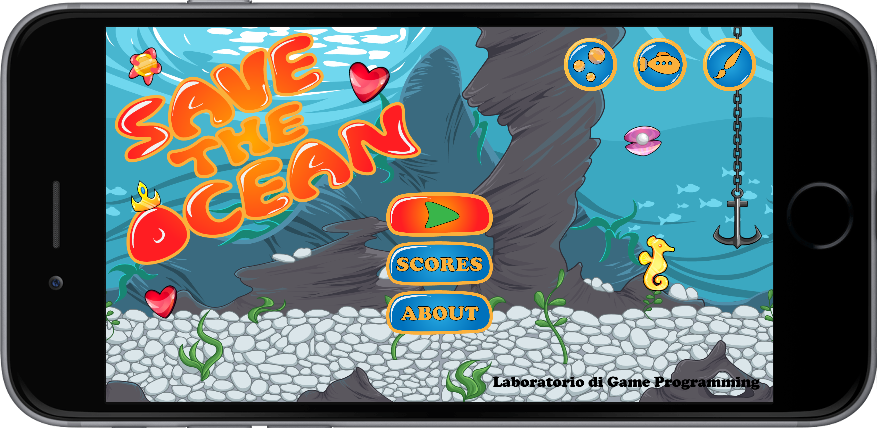
\includegraphics[width=70mm]{Menu.png}\\
Ci sono inoltre tre bottoni secondari: uno realtivo alla scelta delle diverse skin del sottomarino; 

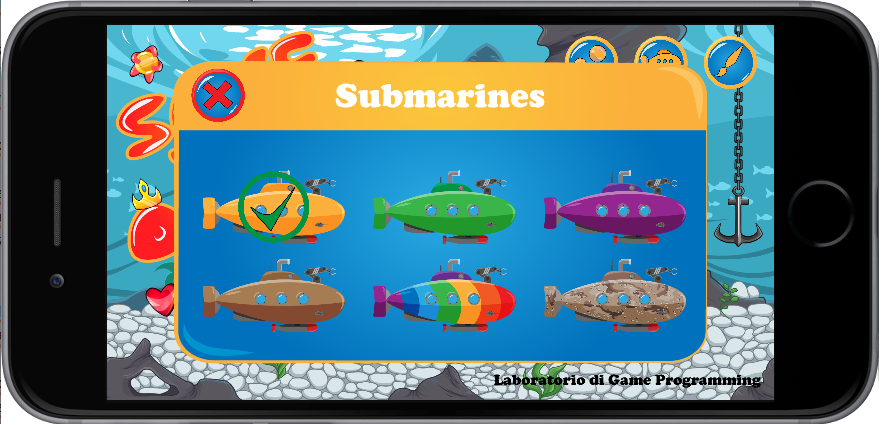
\includegraphics[width=70mm]{skin.png}\\

uno che mostra i vari ambienti di gioco selezionabili; 

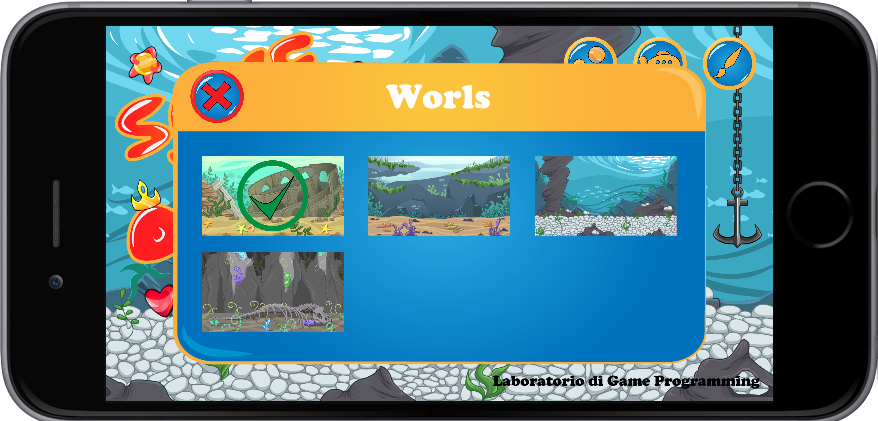
\includegraphics[width=70mm]{ambienti.png}\\
\\
e uno che permette di scegliere il colore delle bolle che usciranno dal sottomarino. 
\\

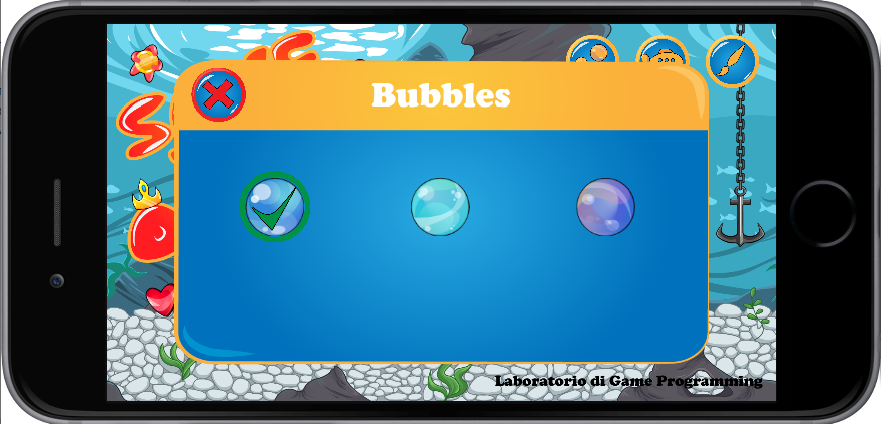
\includegraphics[width=70mm]{bolle.png}\\

\section{Game.lua}
Dopo aver premuto il pulsante play si passa al file "game.lua", in cui vengono realizzati tutti gli oggetti ed il codice relativo alla realizzazione della logica del gioco. 
\subsection{create()}
Nella funzione create(), inzialmente vengono settate le variabili legate al composer: "startTime" è utilizzata per calcolare la velocità dello schermo in base al tempo; "gameSpeed", imposta la velocità iniziale di scorrimento dello schermo (inizialmente gameSpeed = 1). Tale velocità viene aggiornata ogni 1000 ms tramite un listener che chiama la funzione updateGameSpeed. La scelta del valore 1000ms non è casuale, ma è stato inserito in modo tale da non accumulare troppo l'incremento in quel secondo.
\\

Le collisioni tra sottomarino ed oggetti da raccogliere sono gestite a tempo di esecuzione mediante un listener, in questo modo ogni volta che avviene una collisione viene chiamata la funzione onCollision(). 
\\

Il punteggio viene rappresentato mediante un "display object" in cui è stato utilizzato il font di default salvato in una variabile locale in modo tale da renderlo più accessibile in tutte le parti del programma. 

\\
La vita del mare viene creata usando la funzione newProgressView in cui vengono inseriti 3 parametri:
\begin{itemize}
    \item percetuale della vita: rappresentata da un valore all'interno dell'intervallo [0,1] in cui 1 rappresenta il 100 e 0 lo 0. La barra viene creata inizialmente al 100.
    \item posizione della barra a seconda dell'asse X: inizialmente posta al centro dell'asse X (contentCenterX)
    \item posizione della barra a seconda dell'asse Y: 
\end{itemize}
La percentuale di progresso della barra viene gestita da un metodo setProgress inserito all'interno della funzione newProgressView.


\end{document}